\documentclass{article}
% To include code color syntaxing
\usepackage{minted}
% To include images
\usepackage{graphicx}
% To define margins
\usepackage[a4paper,left=2.5cm,right=2.5cm,top=2.5cm,bottom=2.5cm]{geometry}
% To comment multiple lines
\usepackage{comment}
% To use hyperlink
\usepackage{hyperref}
% To write formulas and equations
\usepackage{amsmath}
\usepackage{adjustbox}
\usepackage{caption}
\usepackage{subcaption}
% Setting all hyperlinks color to black, then setting only url colors to blue
\hypersetup{
  colorlinks,
  allcolors=.,
  urlcolor=blue,
}

\begin{document}

\begin{titlepage}
	\begin{center}
		\huge{\bfseries II.2315 – Project : Advanced algorithm and programming} \\
		\rule{16cm}{0.4pt} \\
		\huge{\bfseries Australia - Canberra} \\
		\vspace{3mm}
		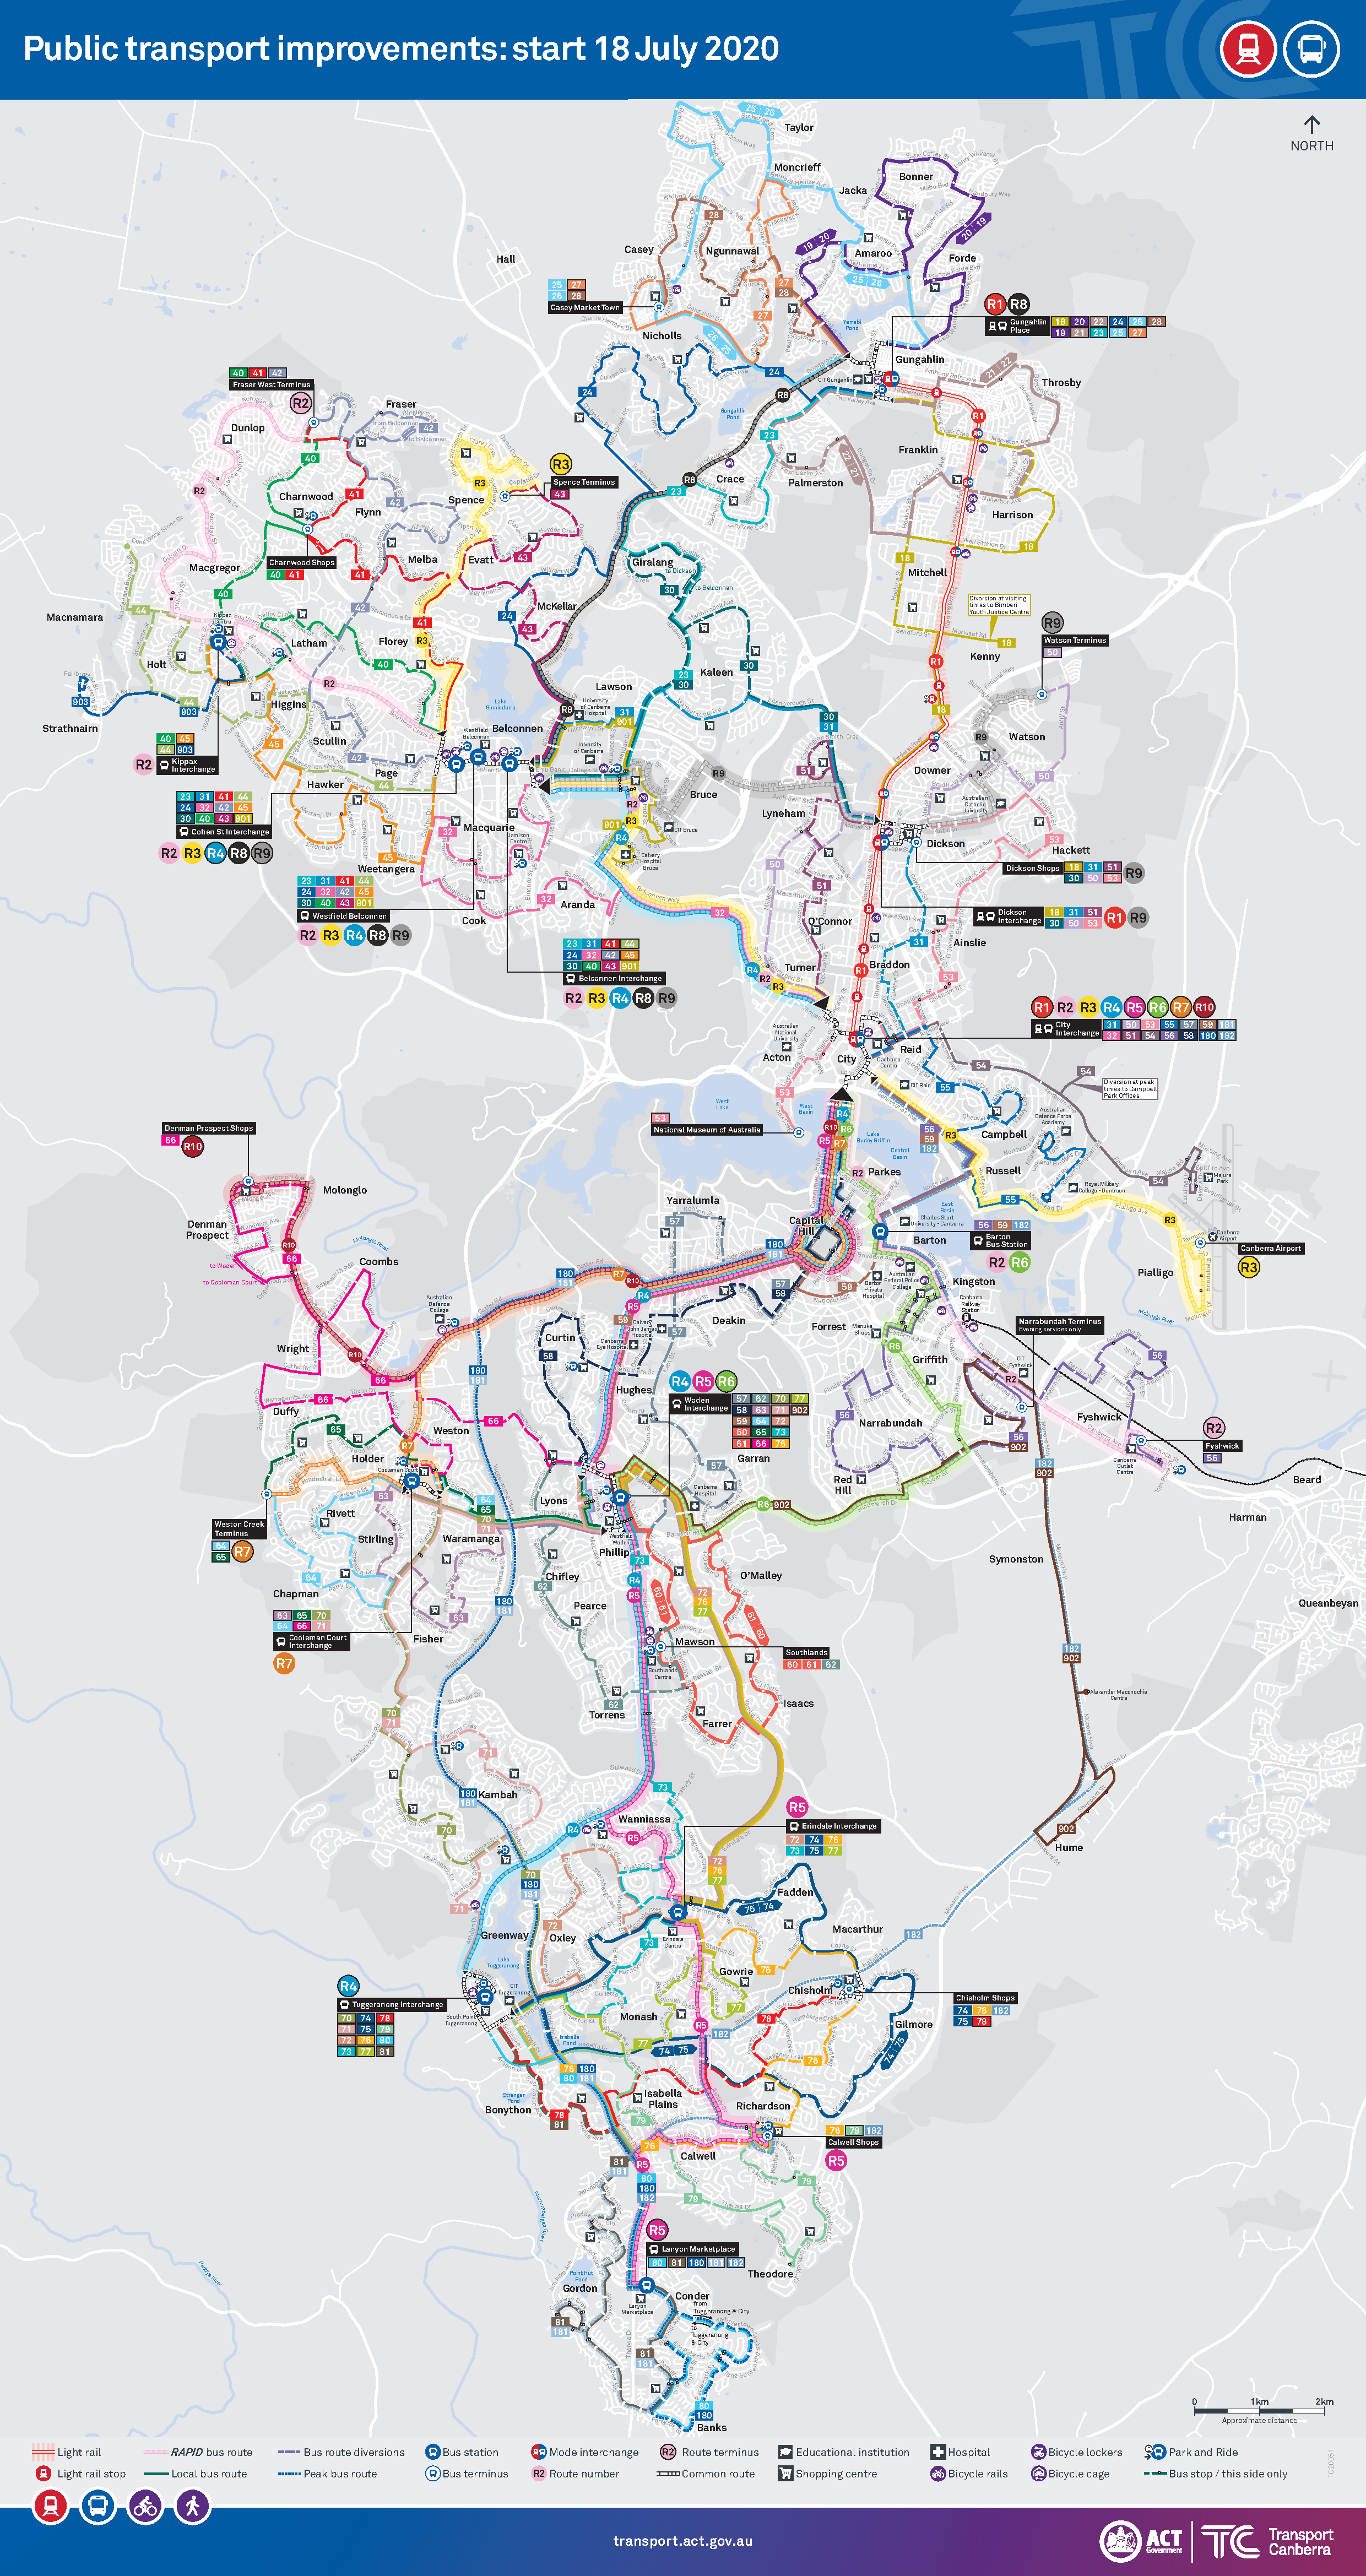
\includegraphics[scale=0.20]{assets/CanberraMap}
		\rule{16cm}{0.4pt} \\
		\vspace{5mm}
		
\includegraphics[scale=0.20]{assets/logoISEP} \\
		\textsc{\large Sarah HEOUAINE - David LAMY-VERDIN - Elia TSO}
		\medbreak
		\textsc{\large 2020 - 2021}
	\end{center}
\end{titlepage}

\renewcommand{\contentsname}{Table of contents}
\tableofcontents
\cleardoublepage

\section{Introduction}

\subsection{City of choice}

	We selected the city of Canberra, capital of Australia, for our project. This city has a total of 2433 stations and 2759 links.
	
\subsection{Goals of the project}

	This project had for first goal to create a graph representing the transport map of Canberra out of mere data. After this graph has been created, we could use it to reach other goals described in the below list:
	
\begin{itemize}
\item[-] Search algorithms \\
Implementation of the Breadth First Search Algorithm \\
Implementation of the Dijkstra Algorithm
\medbreak
\item[-] Applications of those algorithms \\
Searching for shortest paths \\
Splitting the map into clusters
\end{itemize}

	Through this project, optimization also had to be done as searching for shortest paths and splitting into clusters a graph as large as Canberra Transport Map was particularly demanding on resources and took a considerable amount of time.
	
\subsection{Collection of data : GTFS files}
	
	To build our graph, we used data retrieved from \href{https://www.transport.act.gov.au/contact-us/information-for-developers}{Australia Government official website}. This data comes as multiple \textit{.txt} files. After studying them, it has been figured out that we only needed \textit{stops.txt} and \textit{stop\_times.txt} for our project.
	
\begin{figure}[h]
\begin{center}
	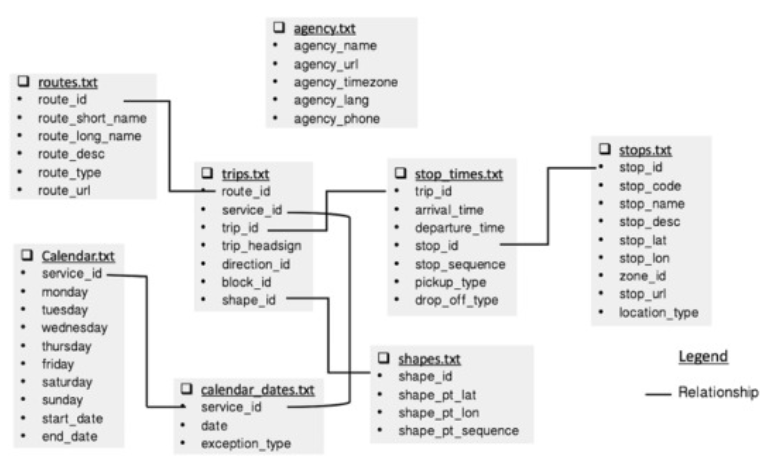
\includegraphics[scale=0.8]{assets/data}
\end{center} 
\caption{Data included in each \textit{.txt} file and relations between them}
\end{figure} 


	Using only those, we could create the stations which are represented in our graph as nodes and we could also link each of them and thus creating our edges.
	
\newpage
	
	The \textit{stops.txt} file provides us with \textit{stop\_id}, \textit{stop\_lat}, \textit{stop\_lon} which gives the number of each station and its geolocation. It will be used to create our nodes. Then the \textit{stop\_times.txt} gives us for each trip \textit{trip\_id} a list of \textit{stop\_id}, which allows us to create our edges. A trip informs about which stations are linked together and in which order as it defines a bus or subway line such as the R3 line of Canberra for example:
	
\begin{figure}[h]
\begin{center}
	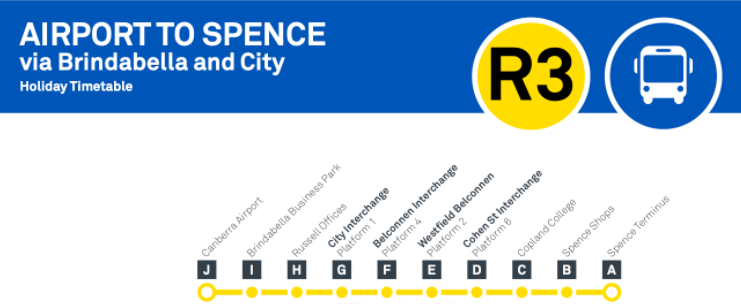
\includegraphics[scale=1]{assets/R3}
\end{center}
\caption{R3 bus line of Canberra}
\end{figure} 

\section{Creation of the graph}

\subsection{Graph}

\mintinline{java}{Graph.java} is the class used for building graphs.
The class contains the three following attributes:

\begin{itemize}
\item[-]\mint[breaklines, breaksymbolleft=]{java}{private Map<Integer, List<DirectedEdge>> map = new TreeMap<Integer,List<DirectedEdge>>()} This \mintinline{java}{Map} is used to store the adjacency lists of every node of our graphs. Each \mintinline{java}{Key} of the \mintinline{java}{Map} designates a node of our graph and the corresponding \mintinline{java}{Value} of the \mintinline{java}{Map} is its adjacency list. We chose to use a \mintinline{java}{Map} over a \mintinline{java}{List} because unlike graphs where nodes labels are consecutive numbers, the stations of Canberra are not labeled consecutively. Therefore, using a \mintinline{java}{Map} makes it easier to look for an adjacency list of a specific station. This would not have been possible with a \mintinline{java}{List}. 
\item[-]\mintinline{java}{private boolean weighted} indicates if the graph is weighted or not.
\item[-]\mintinline{java}{private boolean directed} indicates if the graph is directed or not.
\end{itemize}

	Besides these attributes, \mintinline{java}{Graph.java} also has several methods whose most important ones are the following:

\begin{itemize}
\item[-]\mint[breaklines, breaksymbolleft=]{java}{private void convertTxt(File stopsFile, File stopTimesFile, boolean weighted, boolean directed)}
\item[-]\mint{java}{private void addNodesFromTxt(File stopsFile)}
\item[-]\mint{java}{private void addEdgesFromTxt(File stopTimesFile)}
\item[-]\mint{java}{private void addWeightsFromTxt(File stopsFile)}
\end{itemize}

\begingroup
\setlength{\rightskip}{0pt plus 1 fil}
The first method is used to initialize a graph by calling the other three methods and in the meantime setting the attributes \mintinline[breaklines, breakafter=_]{java}{private boolean weighted} and \mintinline{java}{private boolean directed}.
\endgroup

The other three methods are used to parse \textit{stops.txt} and \textit{stop\_times.txt}, retrieve the data and create the nodes and edges of our graph.

\subsection{Nodes}

For \textit{stops.txt}, each line was containing these informations in this order: stop\_id, stop\_name, stop\_lat, stop\_lon. In order to create our nodes, we had to use the stop\_id as labels for our nodes. To do so, the method \mintinline{java}{private void addNodesFromTxt(File stopsFile)} has been created.

\begin{figure}[h]
\begin{minted}[breaklines]{java}
private void addNodesFromTxt(File stopsFile) throws FileNotFoundException {

	Scanner myReader = new Scanner(stopsFile);
	myReader.nextLine(); // skip headers line
	int stop_id;
		
	while (myReader.hasNextLine()) {
			
		// split the line
		String line = myReader.nextLine();
		String[] arr = line.split(",");
		
		// add the id of the node
		stop_id = Integer.parseInt(arr[0]);
		if (this.map.containsKey(stop_id)) {
			System.out.println("Node in duplicate: " + stop_id);
		} else {
			List<DirectedEdge> list = new ArrayList<DirectedEdge>();
	this.map.put(stop_id, list);
		}
			
	}
}	
\end{minted}
\caption{\mintinline{java}{private void addNodesFromTxt(File stopsFile)}}
\end{figure}


The method takes the \textit{stops.txt} as input and reads every line as a \mintinline{java}{String} using \mintinline{java}{java.util.Scanner}. After splitting the \mintinline{java}{String} using a comma as separator, the method then retrieves the first element of the output array which corresponds to stop\_id and creates a new \mintinline{java}{Entry} to the \mintinline{java}{Graph Map} using the stop\_id as \mintinline{java}{Key} and an empty \mintinline{java}{List<DirectedEdge>} as \mintinline{java}{Value} only if the \mintinline{java}{Graph Map} does not already contain this \mintinline{java}{Key}.

\subsection{Edges}

For \textit{stop\_times.txt}, the information are disposed as below: trip\_id, arrival\_time, departure\_time, stop\_id, stop\_sequence, timepoint. As above, the method \mintinline{java}{private void addEdgesFromTxt(stopTimesFile)} takes \textit{stop\_times.txt} as input and splits each line into an array using commas as separators.

The interesting data in {stop\_times.txt} is both trip\_id and stop\_id. If from a line to the other, the trip\_id is the same, we know that both stations of each line are part of the same bus or subway line and are therefore linked together by an edge.
As the method has to link each line to the previous one to check if the trip\_ id is the same and to create the edge between the two stop\_id, we store the data of the current iteration as well as of the previous iteration.

\newpage

\begin{figure}[H]
\begin{minted}[breaklines]{java}
[...]
if (directed){
	// if we are still in the same trip, then the 2 stations are connected
	if (trip_id.equals(trip_id0)) { 
		if (!this.map.containsKey(stop_id0)) {
			System.out.println("Node does not exist: " + stop_id0);
		} else {
			List<DirectedEdge> edgesList = this.map.get(stop_id0);
			boolean exists = false;
			for (int i = 0; i < edgesList.size(); i++) { // to avoid duplicates
				if (edgesList.get(i).to() == stop_id) {
					exists = true;
					break;
				}
			}
			if (!exists) {
				DirectedEdge newEdge = new DirectedEdge(stop_id0, stop_id, 1);
				edgesList.add(newEdge);
			}
		}
	}
} else if (!directed){
	if (trip_id.equals(trip_id0)) { 
		if (!this.map.containsKey(stop_id0)) {
			System.out.println("Node does not exist: " + stop_id0);
		} else if (!this.map.containsKey(stop_id)) {
			System.out.println("Node does not exist: " + stop_id);
		} else {	
			List<DirectedEdge> edgesList0 = this.map.get(stop_id0);
			List<DirectedEdge> edgesList = this.map.get(stop_id);
			boolean exists = false;
			for (int i = 0; i < edgesList0.size(); i++) { // to avoid duplicates
				if (edgesList0.get(i).to() == stop_id) {
					exists = true;
					break;
				}
			}
			if (!exists) {
				DirectedEdge newEdge0 = new DirectedEdge(stop_id0, stop_id, 1);
				DirectedEdge newEdge = new DirectedEdge(stop_id, stop_id0, 1);
				edgesList.add(newEdge);
				edgesList0.add(newEdge0);
			}
		}
	}
}
[...]
\end{minted}
\vspace*{-10mm}\caption{\mintinline{java}{private void addEdgesFromTxt(File stopTimesFile)}}
\end{figure}

The method then checks if the nodes are actually existing and if they do, it adds the edge to the right adjacency list:

\begin{itemize}
\itemsep0em 
\item[-] only to the source node adjacency list if the graph is directed
\item[-] to both the source and destination nodes adjacency lists if the graph is not directed
\end{itemize}

\newpage

\subsection{Weights}

\begin{figure}[h]
\begin{minted}[breaklines]{java}
[...]
for (Map.Entry<Integer,List<DirectedEdge>> entry : this.map.entrySet()) {
	for (DirectedEdge edge : entry.getValue()) {
		source = edge.from();
		destination = edge.to();
		sourceLat = mapCoord.get(source).getLatitude();
		sourceLong = mapCoord.get(source).getLongitude();
		destinationLat = mapCoord.get(destination).getLatitude();
		destinationLong = mapCoord.get(destination).getLongitude();
		distance = Math.sqrt(Math.pow((destinationLat-sourceLat),2) + Math.pow((destinationLong-sourceLong),2));
		edge.setWeight(distance);
	}
}
[...]
\end{minted}
\caption{\mintinline{java}{private void addWeightsFromTxt(File stopsFile)}}
\end{figure}

\mintinline{java}{private void addWeightsFromTxt(File stopsFile)} is used only if the graph is weighted. It takes \textit{stops.txt} as input and extracts both stop\_lat and stop\_lon for each station to store it into a \mintinline{java}{Map} of \mintinline{java}{Coordinates} which is a \mintinline{java}{Class} that simply has stop\_lat and stop\_lon as attributes. Once the \mintinline{java}{Map} of \mintinline{java}{Coordinates} created, the method calculates the euclidean distance between the starting node and the destination node for every edge of the graph and sets it as weights.

\begin{figure}[h]
\begin{gather*}
  d(a,b) = \sqrt{(a_{lon} - b_{lon})^2 + (a_{lat} - b_{lat})^2}, \\
  \text{where~$a$ is the starting node, and ~$b$ the destination node}
\end{gather*}
\caption{Euclidean distance formula in two dimensions}
\end{figure}

Here is an example of what this method would give for the R3 bus line of Canberra:

\begin{center}
\begin{figure}[h]
\begin{adjustbox}{max width=\textwidth}
\begin{tabular}{ |c|c|c|c|c|c|c| } 
 \hline
 stop\_id: source & stop\_lat: source & stop\_lon: source & stop\_id: destination & stop\_lat: destination & stop\_lon: destination & distance \\ 
 \hline
 3353 & -35.307607 & 149.189463 & 3467 & -35.316348 & 149.190329 & 0.008783793998 \\ 
 \hline
 3467 & -35.316348 & 149.190329 & 3011 & -35.297298 & 149.150267 & 0.04436063958 \\
 \hline
 3011 & -35.297298 & 14.150267 & 3419 & -35.278322 & 149.12815 & 0.02914189879 \\
 \hline
 3419 & -35.278322 & 149.12815 & 5514 & -35.240007 & 149.067995 & 0.07132084723 \\
 \hline
 5514 & -35.240007 & 149.067995 & 5502 & -35.23861 & 149.063546 & 0.004663175956 \\
 \hline
 5502 & -35.23861 & 149.063546 & 940 & -35.24 & 149.060282 & 0.003547646544 \\
 \hline
 940 & -35.24 & 149.060282 & 4072 & -35.21243 & 149.0607 & 0.02757316855 \\
 \hline
 4072 & -35.21243 & 149.0607 & 4091 & -35.194784 & 149.060626 & 0.01764615516 \\
 \hline
 4091 & -35.194784 & 149.060626 & 4807 & -35.200702 & 149.068587 & 0.009919689763 \\
 \hline
 4807 & -35.200702 & 149.068587 & X & X & X & X \\ 
 \hline
\end{tabular}
\end{adjustbox}
\caption{Table of coordinates and distances for edges of the R3 bus line of Canberra}
\end{figure}
\end{center}

\newpage

\section{Pathfinding Algorithm}

\subsection{Breadth First Search}

The Breadth First Search algorithm has been implemented in the \mintinline{java}{BFSSP.java}. The methods of this class have all been made \mintinline{java}{static} as it is not necessary to store any data from one breadth first search to the other. A user would likely use a breadth first search on the graph of their choice and it makes more sense to just create a graph instead of having to create both a graph and a \mintinline{java}{BFS} instance. The method \mintinline{java}{public static List<Integer> bfs(Graph G, int startingNode)} takes a graph and a starting node as parameters and starts a breadth first search.

While doing a breadth first search, we need to store for each node three values:
\begin{itemize}
\item[-]\mintinline{java}{private boolean marked} to know if the node has been reached at some point during the breadth first search
\item[-]\mintinline{java}{private int previous} to know which node precede the node during the breadth first search
\item[-]\mintinline{java}{private int distance} to know the distance separating the node to the starting node of the breadth first search
\end{itemize}

Just as for \mintinline{java}{Map} of \mintinline{java}{Graph.java}, it is more intuitive to use a \mintinline{java}{Map} to store all of these values. One approach could be to use three different \mintinline{java}{Map}, however, to use less memory and make the code more efficient we decided to use a single \mintinline{java}{Map} whose entries would store a tuple of three elements. This tuple contains a \mintinline{java}{boolean} and two \mintinline{java}{int}, and results in the creation of the \mintinline{java}{class} \mintinline{java}{MPD.java}.

\begin{figure}[H]
\begin{minted}[breaklines]{java}
public static List<Integer> bfs(Graph G, int startingNode) {
	List<Integer> path = new ArrayList<Integer>();
	List<Integer> toVisitNodes = new ArrayList<Integer>();
	for (Integer key : G.getMap().keySet()) {
		mapMPD.put(key, new MPD(false, -1, 0.0));
	}
	toVisitNodes.add(startingNode);
	mapMPD.put(startingNode, new MPD(false, -1, 0.0));
	
	if (G.isWeighted()) {
		
		System.out.println("Please consider using Dijkstra Algorithm on weighted graph if you would like to find shortest paths.");
		
	}	
	while (!toVisitNodes.isEmpty()) {

		int currentNode = toVisitNodes.remove(0);
		mapMPD.get(currentNode).marked = true;
		path.add(currentNode);
		
		for (DirectedEdge edge : G.getMap().get(currentNode)) {
			if (!toVisitNodes.contains(edge.to()) && !mapMPD.get(edge.to()).marked) {
				toVisitNodes.add(edge.to());
				mapMPD.get(edge.to()).previous = currentNode;
				mapMPD.get(edge.to()).distance = mapMPD.get(currentNode).distance+1;					
			}
		}
	}
	return path;
}
\end{minted}
\vspace*{-6mm}\caption{\mintinline{java}{public static List<Integer> bfs(Graph G, int startingNode)}}
\end{figure}

When doing the breadth first search, the first thing to do is to check whether the graph given in parameter is weighted or not.  If it is weighted, the method warns the user that the breadth first search cannot be used on weighted graph to look for shortest paths. However, it does not stop the method and still runs the breadth first search, as even though it cannot be used to find shortest paths, it could still be used to discover connected nodes on a weighted graph.

Breadth First Search Algorithm works as follows:
\begin{itemize}
\item[$\bullet$] Adds starting node given in parameter  to \mintinline{java}{toVisitNodes} which is the list of nodes the method is planning to visit
\item[$\bullet$] Sets the first element of \mintinline{java}{toVisitNodes} as the current node and removes it from list ; sets its \mintinline{java}{MPD.marked} attribute to \mintinline{java}{true}
\item[$\bullet$] For every neighbor of the current node, adds it to \mintinline{java}{toVisitNodes} if it is not marked yet and if it is not contained in \mintinline{java}{toVisitNodes}
\item[$\bullet$] Loop until \mintinline{java}{toVisitNodes} is empty, meaning there is not any remaining connected node that has yet to be visited
\end{itemize}

\subsection{Dijkstra Algorithm}

The Breadth First Search algorithm has been implemented in the \mintinline{java}{Dijkstra.java}. For the same reasons as the breadth first search, all of the methods of Dijkstra Algorithm have been made static. The Dijkstra Algorithm uses the exact same attributes as the Breadth First Search Algorithm which are \mintinline{java}{marked}, \mintinline{java}{previous}, \mintinline{java}{distance}, all contained in \mintinline{java}{MPD}. The advantage the Dijstra Algorithm has over the Breadth First Search Algorithm is that it can look for shortest paths even in the graph with weighted edges.

Dijkstra Algorithm works as follows:

\begin{itemize}
\item[$\bullet$] Adds starting node given in parameter  to \mintinline{java}{toVisitNodes} which is the list of nodes the method is planning to visit
\item[$\bullet$] Sets the closest element of \mintinline{java}{toVisitNodes} (element with the shortest distance) as the current node and removes it from list ; sets its \mintinline{java}{MPD.marked} attribute to \mintinline{java}{true}
\item[$\bullet$] For every neighbor of the current node: 
\\ Updates the distance by replacing it if the distance is shorter than previously 
\\ Adds it \mintinline{java}{toVisitNodes} only if it is not marked yet and if it is not contained in \mintinline{java}{toVisitNodes}
\item[$\bullet$] Loops until \mintinline{java}{toVisitNodes} is empty, meaning there is not any remaining connected node that has yet to be visited
\end{itemize}

\subsection{Shortest paths}

Assuming one of the aforementioned algorithms has already been launched for the starting node of the shortest path the user is looking for, the shortest path can then first be printed.

Before printing a path, it is necessary to make sure this path actually exists. In order to do so, the method \mintinline{java}{public static boolean hasPathTo(int destination)} has been implemented. It simply returns a boolean indicating if a path exists or not. It can be done easily as the \mintinline{java}{marked} attribute of \mintinline{java}{MPD} solely serves this purpose and just returning its value does the trick.

\mintinline{java}{public static printShortestPath(int startingNode, int destinationNode)} first checks if the path exists using \mintinline{java}{hasPathTo()}. If it does not, the code warns the user by printing a message. Another check done by the method is the egality of \mintinline{java}{startingNode} and \mintinline{java}{destinationNode}. If these nodes are the same, there is no need to continue.

Once these checks done, if a path exists and the starting node is distinct from the destination node, the algorithm starts looking for the shortest path. It does so by browsing \mintinline{java}{MPD.previous} attribute starting from the destination node and going all the way back to the starting node. As the path is discovered from destination to start, the code builds the path backwards.

To check if our paths are built correctly, we used the \href{https://www.transport.act.gov.au/getting-around/journey-planner}{Australia Government Official Website Journey Planner} . After using our algorithm to print a shortest path, we used the \textit{stops.txt} file to find the name of the stations and checked if they were the same as in the journey planner.

\newpage
Here is below what the console returns for \mintinline{java}{printShortestPath(6155,6104)} for \mintinline{java}{dijkstra} on a weighted digraph:

\begin{minted}[breaklines]{java}
The path from 6155 to node 6104 is 6155 4754 4756 4758 4934 4919 6092 6006 6008 6070 6053 6055 6057 6059 6074 6341 6182 6184 7010 7012 5085 6028 6026 6024 6038 6035 6033 6032 6049 6048 6154 6129 6102 6104
\end{minted}

\begin{figure}[h]
\centering
\begin{subfigure}{.5\textwidth}
  \centering
  \begin{tabular}{ |c|c| } 
 \hline
 Station ID & Station name \\ 
 \hline
 6155 & Bimberi Centre \\
 \hline
 6104 & Bernard Heinze Av before Crackajack Way \\
 \hline
 4754 & Sandford St after Flemington Rd \\
 \hline
 4756 & Sandford St opp 2nd Kemble Crt \\
 \hline
 4758 & Hoskins St opp Lysaght St \\
 \hline
 4934 & Hoskins St before Dacre St \\
 \hline
 4919 & Hoskins St before Well Station Dr \\
 \hline
\end{tabular}
  \caption{Table of stations ID and names}
\end{subfigure}%
\begin{subfigure}{.5\textwidth}
  \centering
  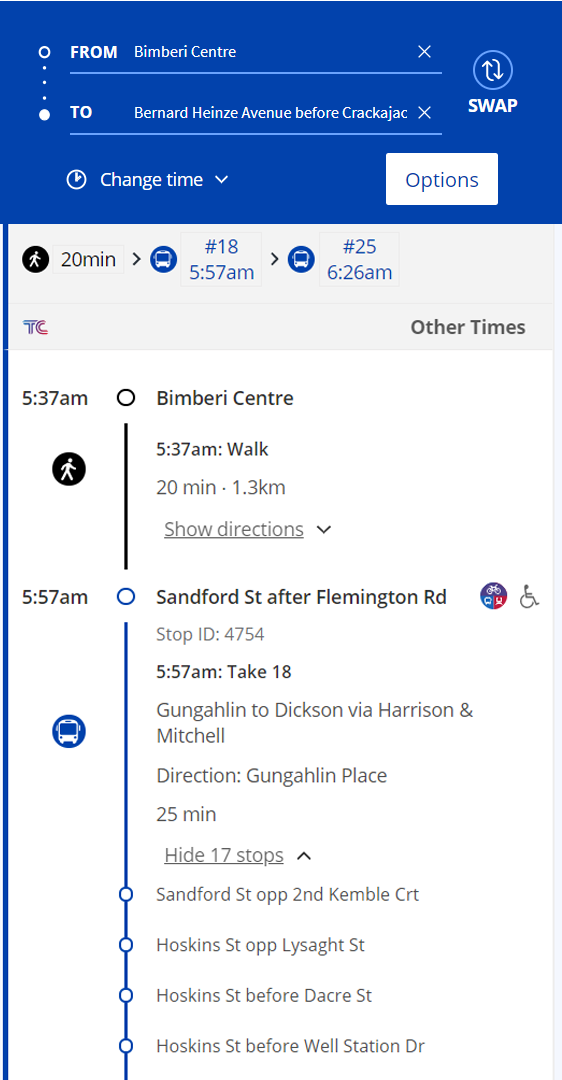
\includegraphics[width=.7\linewidth]{assets/JourneyPlanner}
  \caption{Journey Planner Path}
\end{subfigure}
\caption{Comparison between found path and official journey planner path}
\end{figure}

Using the \href{https://www.transport.act.gov.au/journey-planner-map?flat=-35.22262&flng=149.15615&fname=Bimberi%20Centre&fid=pt_pub|AU_ACT_Canberra|6155&fsrc=SKEDGO&tlat=-35.157483&tlng=149.117915&tname=Bernard%20Heinze%20Avenue%20before%20Crackajack%20Way,%20Canberra,%20ACT,%20Australia&tid=node/6357446892&tsrc=PELIAS&type=0&time=1610299291}{Australia Government Official Website Journey Planner}, we looked for the path from Bimberi Centre to Bernard Heinze Av before Crackajack Way which is no other than the path from station 6155 to 6104 the console printed. Looking at the table provided above and the screenshot of the journey planner, we can see that the first stations returned by the dijkstra are exactly the same as the stations given by the journey planner.

\newpage

\section{Graph Clustering}

\subsection{Calculate the edge-betweenness}

A graph can be cut in many disconnected components also called clusters. As a cluster has to be completely disconnected from an other, it has been decided that the clusters would be created on undirected graphs. Indeed, as all the lines of a bus or subway can be ridden in a direction and the opposite one, if the code was to remove edges to form clusters, it makes more sense to remove an edge in both directions simultaneously.

In order to create clusters, it is necessary to calculate the edge-betweenness of all the edges inside our graph beforehand. To do so, a method named \mintinline{java}{updateCountSP(Graph G)} has been implemented inside \mintinline{java}{DijkstraSP.java}. This method looks for all the shortest paths in the graph and updates the edge-betweenness of every edge everytime they are being taken.

The first algorithm we came out with is:

\begin{itemize}
\item[$\bullet$] Iterates through all the nodes constituting the graph
\item[$\bullet$] Sets the current node as the starting node
\item[$\bullet$] Starts a dijkstra with the starting node as a parameter
\item[$\bullet$] For every destination node reached while doing dijkstra: looks for the path using \mintinline{java}{previous} by doing the same as in \mintinline{java}{printShortestPath()}
\item[$\bullet$] While looking for the path, adds $1$ to the edge-betweenness of the edge connecting the previous node and the current node
\item[$\bullet$] Loop until all the nodes of the graph have been used as starting nodes, meaning every shortest path has been created
\end{itemize}

\medbreak

Because we have to do a dijkstra for every starting node and have to create an edge-beweenness between every pair of nodes of the graph, this algorithm takes a lot of time and resources to execute.
In order to make the algorithm more efficient, we have come up  with the following idea:

\begin{itemize}
\item[$\bullet$] Creates a list \mintinline{java}{unvisited} with all the nodes constituting the graph
\item[$\bullet$] Iterates through all the nodes in \mintinline{java}{unvisited}
\item[$\bullet$] Sets the current node as the starting node
\item[$\bullet$] Starts a dijkstra with the starting node as a parameter
\item[$\bullet$] For every node inside \mintinline{java}{unvisited}: looks for the path (from starting to destination) using \mintinline{java}{previous} by doing the same as in \mintinline{java}{printShortestPath()} and in the meantime, looks for the backward path (from destination to starting)
\item[$\bullet$] While looking for the path, adds $1$ to the edge-betweenness of the edges connecting the previous node and the current node (both the edge previous node $\rightarrow$ current node and the edge current node $\rightarrow$ previous node as the graph is undirected) because we are constructing the path and backwarding path at the same time
\item[$\bullet$] Removes the starting node from \mintinline{java}{unvisited}
\item[$\bullet$] Stops when done iterating through all the nodes of the graph, meaning every shortest path has been created
\end{itemize}

\medbreak

This optimization comes from the observation that, since the graph is undirected, given two stations $a$ and $b$, the path $a \rightarrow b$ and the path $b \rightarrow a$ are necessarily the same but in reverse. That means, because we changed the code to build the paths heading to $a$ while it builds the paths heading from $a$, there is no need to build paths heading to $a$ again in the following iterations (for example $b \rightarrow a$, $c\rightarrow a$ etc.)

\newpage

\subsection{Finding clusters}

In order to find our clusters and count them, the method \mintinline{java}{public static void findClusters(Graph g)} in the class \mintinline{java}{GraphClustering.java} has been created. 

\begin{figure}[h]
\begin{minted}[breaklines]{java}
public static void findClusters(Graph g) {
	System.out.println("...Searching for clusters...");
	for (int key : g.getMap().keySet()) {
		marked.put(key, false);
	}
	
	int i = 0;
	for (int node : g.getMap().keySet()) {
		if (marked.get(node) == false) {
			Cluster cluster = new Cluster();
			List<Integer> dijkstraOutput = DijkstraSP.dijkstra(g, node); // dijkstra will go through each connected component
			for (int dijkstraNode : dijkstraOutput) {
				cluster.addNode(dijkstraNode);
				marked.put(dijkstraNode, true);
			}
			clusters.put(i++,  cluster);
		}
	}
}
\end{minted}
\caption{\mintinline{java}{public static void findClusters(Graph g)}}
\end{figure}
The method uses a \mintinline{java}{Map} \mintinline{java}{marked} which takes a node label as a key and a boolean as the value. It is initialized by creating entries for all the nodes in the graph and setting their values to false. The method then iterates through all the nodes of the graph, if a node is not marked yet, it launches a dijkstra with this node as the starting node. Afterwards, it stores all the nodes by the dijsktra in a new \mintinline{java}{Cluster} and marks them as visited in \mintinline{java}{marked}. It finally adds the \mintinline{java}{Cluster} to a \mintinline{java}{static List<Cluster>} attribute of \mintinline{java}{GraphClustering.java}.

\newpage

\subsection{Creating clusters}

\mintinline{java}{public static void createClusters(Graph G, int n)} allows a user to create as many clusters as given in argument in the desired graph. It takes the graph that has to be divided into clusters as well as the number of clusters wished as input.
The algorithm implemented by this method is the following one:

\begin{itemize}
\item[$\bullet$] Updates the edge-betweenness of all the edges by calling \mintinline{java}{updateCountSP(Graph G)}
\item[$\bullet$] Removes the edge with the highest edge-betweenness
\item[$\bullet$] Looks for the clusters and their numbers by calling \mintinline{java}{findClusters(Graph G)}
\item[$\bullet$] Stops when \mintinline{java}{n} clusters have been found or when there is not any edge left to remove from the graph
\end{itemize}

\medbreak

Here is below a table comparing the execution time of \mintinline{java}{createClusters()} before and after optimization for several number of clusters:

\begin{center}
\begin{figure}[h]
\begin{center}
\begin{tabular}{ |c|c|c|c|c| } 
 \hline
 Number of clusters created & 2 & 4 & 8 & 16 \\ 
 \hline
 Number of edges removed & 4 & 32 & 55 & 99 \\
 \hline
 Time elapsed before optimization & 06:24 & 21:10 & 27:46 & 32:01 \\
 \hline
 Time elapsed after optimization & 04:52 & 16:31 & 19:55 & 24:29 \\
 \hline
\end{tabular}
\end{center}
\caption{Table of elapsed times before and after optimizations when creating $n$ clusters}
\end{figure}
\end{center}

It can be seen that the optimization indeed makes the code more efficient as the execution time ends up being reduced. For 2 clusters, the reduction is only about $01:30$ but as we increase the number of desired clusters, the reduction ends up being more and more important reaching about 8 minutes for both 8 and 16 clusters.

These tests have been run on a computer using Windows 10 with the following specifications:
\begin{itemize}
\item[-] AMD Ryzen 5 2600U QuadCore 2.00GHz
\item[-] 8GB RAM 2400MHz
\end{itemize}

\medbreak

Below lies an example of what the console return when we create 4 clusters.

\begin{minted}[breaklines]{java}
...Updating edge-betweenness of all edges...
Edge (2039;2041) with 326112 SP going through will be removed

...Searching for clusters...
Cluster 1 (632 stations): 2 1808 1908 [...] 2042 2654 2041

Cluster 2 (516 stations): 201 1250 1252 [...] 1271 1265 1270

Cluster 3 (832 stations): 300 3234 3236 [...] 4180 4938 4182 

Cluster 4 (453 stations): 401 403 4323 [...] 4103 4105 4807 
4 cluster(s) have been found 

32 edges have been removed
Execution time : 17 min 52 s
\end{minted}

We can see that it returns some useful information. At each iteration, it displays the edge that is going to be removed with the amount of shortest paths going through. At each iteration, it also displays the number of clusters found, the clusters and their respective stations. Finally, at the end of the process, it prints the number of removed edges as well as the execution time.

\newpage

\section{Possible improvements}

To reduce the execution time of \mintinline{java}{updateCountSP(Graph G)}, we have thought of other ideas but could not have the time to implement all of them. The first two ideas come from the fact that in a shortest path, every intermediary path is also a shortest path to the intermediary node.
\begin{itemize}
\item[$\bullet$] Knowing that, it means that when we are building a shortest path from a starting node to a destination node, we are actually building as many shortest paths as the number of nodes we have reached. Everytime the code reaches a node while building a shortest path, it also builds the shortest path to the node we have reached. The idea is therefore to take these intermediary paths into consideration and not build these paths again in the next iterations. If we could implement it, it would reduce the number of iterations.
\item[$\bullet$] Coming from the same observation, the second idea is that when building a path, if we reach a node that already has a known path, there is no need to continue building, we could just concatenate the path. \\ \\
The issue with both of these ideas is that in our algorithm, we do not store any path (as it would use too much memory), we just build them and update the edge-betweenness for the edges taken. It is still possible to do but it is way trickier. One of the solutions for the second idea would be to use a \mintinline{java}{Map<Integer,List<DirectedEdge>} but it would be at the cost of more memory usage. Every time we reach a node, we check, thanks to this list, if the path already exists, if it is the case, we "concatenate" the path which is fairly simple as we just have to add $1$ to the edge-betweenness of every edge in the \mintinline{java}{List<DirectedEdge>} of the corresponding \mintinline{java}{Map.Entry}.
\item[$\bullet$] The last idea we came up with comes with the observation that when removing an edge, not all the shortest paths are destroyed but only some of them. If we managed to identify which shortest paths are intact, we would not have to calculate the edge-betweenness of the edges taken by these shortest paths again. We would only have to update the edge-betweenness for the edges taken by destroyed shortest paths (remove $1$ to edge-betweenness) or taken by new shortest paths after the previous one has been destroyed (add $1$ to edge-betweenness). However, to implement this, it would be necessary to store all the shortest paths, thing we do not want as it consumes too much memory.
\end{itemize}

\section{Conclusion}

This project was really interesting to work on as it made use of the different algorithms we studied and how they could be used to find shortest paths, find connected components, create clusters and so on. As the graph we worked on was also rather large, it was interesting to think about ways of optimization of our algorithms in order to use as less memory as possible and to shorten as much as possible the execution time.

\newpage

\thispagestyle{empty}
\listoffigures

\end{document}
